\section{DIS projections for LHC far-forward experiments}
\label{sec:dis_pseudodata}

Here we describe the procedure adopted in order 
to generate projections for the kinematic coverage
and experimental uncertainties associated to  measurements
of neutrino-nucleus scattering at the LHC far-forward experiments.
%
First, we summarise the theoretical description of differential
neutrino scattering in terms of DIS structure functions and highlight
their PDF sensitivity.
%
Second, we present an  overview of the operative and proposed
LHC far-forward neutrino detectors that
will be considered in the present study and indicate their
main acceptance and performance parameters.
%
By convoluting the expected muon neutrino fluxes
with the acceptance and scattering rates of each
of these detectors,
we evaluate the foreseen event yields in bins of $x$, $Q^2$,
and $E_\nu$ and therefore the associated statistical uncertainties.
%
We also estimate how the systematic uncertainties in the measurement
of final-state variables affects the experimental covariance matrix. 

\subsection{Neutrino DIS revisited}

The double-differential cross-section for neutrino-nucleus charged-current scattering,
see~\cite{Candido:2023utz} and references therein,
is expressed in terms of 
independent structure functions $F_2^{\nu A}$, $xF_3^{\nu A}$
and $F_L^{\nu A}$:
\be
\label{eq:neutrino_DIS_xsec_FL}
\frac{d^2\sigma^{\nu A}(x,Q^2,y)}{dxdy} =  \frac{G_F^2s/4\pi}{\lp 1+Q^2/m_W^2\rp^2}\lc Y_+F^{\nu A}_2(x,Q^2) - y^2F^{\nu A}_L(x,Q^2) +Y_- xF^{\nu A}_3(x,Q^2)\rc  \, ,
\ee
where $Y_\pm = 1 \pm (1-y)^2$ and with a counterpart expression for anti-neutrino scattering,
\be
\label{eq:antineutrino_DIS_xsec_FL}
\frac{d^2\sigma^{\bar{\nu} A}(x,Q^2,y)}{dxdy} =  \frac{G_F^2s/4\pi}{\lp 1+Q^2/m_W^2\rp^2}\lc Y_+F^{\bar{\nu} A}_2(x,Q^2) - y^2F^{\bar{\nu} A}_L(x,Q^2) -Y_- xF^{\bar{\nu} A}_3(x,Q^2)\rc  \, ,
\ee
where $s=2m_N E_\nu$ being the neutrino-nucleon center of mass energy squared, $m_N$ is the nucleon mass,
$E_\nu$ is the incoming neutrino energy,
and the inelasticity is $y=Q^2/(2x m_n E_{\nu})$.
%
Structure functions depend only on $x$ and $Q^2$ while the differential
cross-section depends also on the neutrino energy $E_\nu$, or alternatively
on the inelasticity $y$.
%
Further, structure functions $F^{\nu A}_i(x,Q^2)$ and $F^{\bar{\nu} A}_i(x,Q^2)$ depend on the nuclear target $A$ entering
for the neutrino scattering through the nuclear modifications of the proton PDFs.

Eqns.~(\ref{eq:neutrino_DIS_xsec_FL}) and~(\ref{eq:antineutrino_DIS_xsec_FL}) are valid provided
the hadronic 
invariant mass $W$  is above the resonance threshold,
\be
W^2 = \lp m_N^2 + Q^2 \frac{(1-x)}{x} \rp \gsim \lp 2\,{\rm GeV} \rp^2\, ,
\ee
and in addition here we  restrict ourselves to the DIS region with perturbative momentum
transfers $Q^2$, such that
 structure functions are decomposed as
\be
\label{eq:sfs_pqcd}
 F^{\nu A}_i(x,Q^2) = \sum_{j=q,\bar{q},g}\int_x^1 \frac{dz}{z}\, C_{i,j}^{\nu N}(z,\alpha_s(Q^2))f^{(A)}_j\lp \frac{x}{z},Q^2\rp \, , \quad i = 2,3,L \, .
 \ee
%
in terms of a convolution of partonic scattering cross-sections  $C_{i,j}^{\nu N}(x,\alpha_s)$ and
of process-independent PDFs $f^{(A)}_j\lp x,Q^2\rp$.
%
Specifically, in this work we impose that $Q^2\ge 2$ GeV$^2$.
%
A similar expression holds for charm production~\cite{Faura:2020oom}, which requires
accounting also for charm mass effects~\cite{Gao:2017kkx}.
 %
We discuss in Sect.~\ref{sec:settings} the theoretical
settings adopted~\cite{Candido:2022tld,yadism,Candido:2023utz,Carrazza:2020gss} to
evaluate predictions for
neutrino DIS structure functions
and differential cross-sections,
Eqns.~(\ref{eq:neutrino_DIS_xsec_FL}),~(\ref{eq:antineutrino_DIS_xsec_FL}), and~(\ref{eq:sfs_pqcd}),
in the kinematics covered by LHC neutrinos.

Different neutrino structure functions provide complementary sensitivity
 to the partonic flavour decompositions of nucleons.
 %
 To illustrate this sensitivity, consider a leading order  calculation
 for a proton target with $n_f=4$ active quark flavours,
a diagonal CKM matrix and no heavy quark mass effects.
 %
 The resulting $F_2^{\nu p}$ and $xF_3^{\nu p}$ structure functions read
 \bea
 F_2^{\nu p}(x,Q^2) &=& 2x\lp f_{\bar{u}} + f_{d} + f_{s} + f_{\bar{c}} \rp(x,Q^2) \, , \nonumber  \\
 F_2^{\bar{\nu} p}(x,Q^2) &=& 2x\lp f_u + f_{\bar{d}} + f_{\bar{s}} + f_c \rp(x,Q^2) \, , \label{eq:neutrinoSFs_proton} \\
 xF_3^{\nu p}(x,Q^2) &=& 2x\lp -f_{\bar{u}} + f_d +f_s - f_{\bar{c}}\rp(x,Q^2)  \, , \nonumber\\
 xF_3^{\bar{\nu} p}(x,Q^2) &=& 2x\lp f_u - f_{\bar{d}} -f_{\bar{s}} + f_{c}\rp(x,Q^2) \, . \nonumber
 \eea
 The corresponding expressions for a neutron target are obtained from isospin symmetry
 \bea
 F_2^{\nu n}(x,Q^2) &=& 2x\lp f_{\bar{d}} + f_{u} + f_{s} + f_{\bar{c}} \rp(x,Q^2) \, , \nonumber  \\
 F_2^{\bar{\nu} n}(x,Q^2) &=& 2x\lp f_d + f_{\bar{u}} + f_{\bar{s}} + f_c \rp(x,Q^2) \, , \label{eq:antineutrinoSFs_neutron} \\
 xF_3^{\nu n}(x,Q^2) &=& 2x\lp -f_{\bar{d}} + f_u +f_s - f_{\bar{c}}\rp(x,Q^2)  \, , \nonumber\\
 xF_3^{\bar{\nu} n}(x,Q^2) &=& 2x\lp f_d - f_{\bar{u}} -f_{\bar{s}} + f_{c}\rp(x,Q^2) \, , \nonumber
 \eea
 while for an isoscalar, free-nucleon target denoted by $N$ one has
 \bea
 F_2^{\nu N}(x,Q^2) &=& 2x\lp f_{u^+} + f_{d^+} + 2f_s + 2f_{\bar{c}} \rp(x,Q^2) \, , \nonumber  \\
 F_2^{\bar{\nu} N}(x,Q^2) &=& 2x\lp f_{u^+} + f_{d^+} + 2f_{\bar{s}} + 2f_c \rp(x,Q^2) \, , \label{eq:neutrinoSFs_isoscalar} \\
 xF_3^{\nu N}(x,Q^2) &=& 2x\lp f_{u^-} + f_{d^-} +2f_s - 2f_{\bar{c}}\rp(x,Q^2)  \, , \nonumber\\
 xF_3^{\bar{\nu} N}(x,Q^2) &=& 2x\lp   f_{u^-} + f_{d^-}-2f_{\bar{s}} +2 f_{c}\rp(x,Q^2) \, , \nonumber
 \eea
 in terms of the valence and sea PDF combinations defined by
 \be
 f_{q^+} (x,Q^2)\equiv \lp f_{q}+f_{\bar{q}}\rp(x,Q^2) \, , \qquad
 f_{q^-} (x,Q^2)\equiv \lp f_{q}- f_{\bar{q}}\rp(x,Q^2) \, .
 \ee
 We note that, even for isoscalar targets, separate measurements
 for neutrinos and antineutrinos will not be equivalent, since in general
 the strange and charm sea asymmetries $f_{s^-}$ and
 $f_{c^-}$ are not expected to vanish.

 In the projections presented in this work, when interpreting the LHC neutrino structure
 functions in terms of proton PDFs, we will assume a isoscalar free-nucleon target and neglect
 nuclear PDF modifications, along the lines of Eq.~(\ref{eq:neutrinoSFs_isoscalar}).
 %
 On the other hand, when evaluating structure functions
 for a tungsten (W) target, we keep into account both
 nuclear corrections and that
 the target is not isoscalar when evaluating the physical observables.
 %
 We point out that accounting for nuclear modifications in a global proton
 PDF fit is possible by means of the procedure developed
 in~\cite{Ball:2020xqw,Ball:2018twp}.

 It is illustrative to compare the PDF dependence of neutrino structure functions
 at LO with that of their counterparts for neutral-current
 scattering with a charged lepton projectile.
 %
 Within the same assumptions, for energies below
 the $Z$-boson mass, $Q^2 \ll m_Z^2$, the corresponding
 partonic decomposition is
 the 
 \bea
 F_2^{\ell p}(x,Q^2) &=& x\lp \frac{4}{9}\lc f_{u^+} + f_{c^+}\rc
 + \frac{1}{9}\lc f_{d^+} + f_{s^+}\rc\rp(x,Q^2) \, , \nonumber  \\
 F_2^{\ell n}(x,Q^2) &=& x\lp \frac{4}{9}\lc f_{d^+} + f_{c^+}\rc
 + \frac{1}{9}\lc f_{u^+} + f_{s^+}\rc\rp(x,Q^2) \, ,\label{eq:NC_chargedlepton}   \\
 F_2^{\ell N}(x,Q^2) &=& x\lp \frac{5}{18}\lc f_{u^+} + f_{d^+}\rc
 + \frac{1}{9} f_{s^+} + \frac{4}{9} f_{c^+} \rp(x,Q^2) \, , \nonumber  
 \eea
 with $xF_3$ being negligible in this region below the $Z$-pole.
 %
 Eq.~(\ref{eq:NC_chargedlepton}) showcases the complementarity between
 neutrino and charged-lepton DIS in terms of sensitivity
 to the different flavour PDF decomposition.

 \subsection{Far-forward neutrino detectors at the LHC}
 \label{sec:neutrinoDetectors}

 As we discuss below, the calculation of differential neutrino scattering event rates
 at the LHC far-forward detectors requires two main ingredients: the energy
 and flavour dependence of the incoming neutrino flux crossing
 the detector fiducial volume, on the one hand,
 and the scattering rates within the same fiducial volume, on the other hand.
 %
 In this section, we summarise the main features of each of the ongoing and future
 far-forward detectors considered in this study, in particular concerning
 their acceptance, geometry, and neutrino detection method.
 %
 We also indicate the expected performance of the three FPF detectors
 and how this translates into the dominant experimental systematic
 uncertainties.
 %
 Since for the projection studies considered in this work we focus on muon
 neutrino scattering, we will focus the subsequent discussion on the detection
 performance of this neutrino flavour.

 Table~\ref{tab:FPF_experiments} indicates
 the rapidity coverage, target material,
 muon neutrino acceptance, and the identification and reconstruction performance
 for each of the far-forward LHC neutrino experiments considered
 in this work.
 %
 More details of the information listed in this table is provided
 in the following.

  %-----------------------------------------------------------------
\begin{table}[t]
  \centering
  \small
  \renewcommand{\arraystretch}{1.50}
\begin{tabularx}{\textwidth}{Xccccc}
\toprule
Detector &  Rapidity &  Target & Charged Lepton ID & Acceptance  & Performance \\
\midrule
\midrule
\multirow{2}{*}{FASER$\nu$}  &  \multirow{2}{*}{ $|\eta_\nu| \le 8.5$}  &   Tungsten  & \multirow{2}{*}{muons}      &   $E_\ell \gsim 100$ GeV   &    \multirow{2}{*}{n/a}       \\
  &   &   (1.1 ton)  &       &  $\tan \theta_\ell \lsim 0.5$   &         \\
\midrule
\multirow{2}{*}{SND@LHC}  & \multirow{2}{*}{ $7.2 \le \eta_\nu \le 8.4$}   &  Tungsten   &   \multirow{2}{*}{n/a}    &  $E_\mu \gsim 20 $ GeV     &    \multirow{2}{*}{n/a}    \\
  &    &  (0.83 ton)   &  &  $\theta_\mu \lsim 0.15, \theta_e \lsim 0.5$         &       \\
\midrule
\midrule
\multirow{3}{*}{FASER$\nu$2}  & \multirow{3}{*}{ $|\eta_\nu| \le 8.5$}  & \multirow{2}{*}{Tungsten}    &   \multirow{3}{*}{muons}     &   $E_\ell \gsim 100$ GeV  &    $\delta E_\ell \sim 30\% $     \\
  &   &  \multirow{2}{*}{(20 ton)}   &       &  $\tan \theta_\ell \lsim 0.5$   &   $\delta \theta_\ell \sim 1$ mrad      \\
  &   &     &       &  reconstructed $E_h$ \& charm ID   &  $\delta E_h \sim 30\%$        \\
\midrule
\multirow{3}{*}{AdvSND~(far)}  &   \multirow{3}{*}{ $7.2 \le \eta_\nu \le 8.4$}  &
\multirow{2}{*}{Tungsten}   &   \multirow{3}{*}{muons}    &  $E_\mu \gsim 20 $ GeV  & \multirow{3}{*}{n/a}          \\
  &   &   \multirow{2}{*}{(5 ton)}  &        & $\theta_\mu \lsim 0.15, \theta_e \lsim 0.5$     &           \\
  &   &     &       &  reconstructed $E_h$   &           \\
\midrule
\multirow{3}{*}{FLArE}  & \multirow{3}{*}{tbd} & \multirow{2}{*}{Liquid Argon}  & \multirow{3}{*}{ maybe muons}  &  $E_\mu \lsim 2$ GeV, $E_e \lsim 1$ TeV    &    $\delta E_e \sim 5\% $ \\
&   &  \multirow{2}{*}{(10 ton)}   &   & $\theta_\mu \lsim 0.4$, $\theta_e \lsim 0.5$ &    $\delta \theta_e \sim 15 $ mrad   \\
 &   &     &  & reconstructed $E_h$  &    $\delta E_h \sim 30\% $   \\
  \bottomrule
\end{tabularx}
\vspace{0.2cm}
\caption{\small For each of the far-forward LHC neutrino experiments considered
  in this work, we indicate their neutrino pseudo-rapidity coverage, target material, whether
  they can identify the sign of the outgoing charged lepton,
  the acceptance for the charged lepton and hadronic final state,
  and the expected reconstruction performance.
  %
  We consider separately acceptance and performance for electron and muon
  neutrinos, while tau neutrinos have lower production rates and are not considered in this study.
  %
  See the description of each experiment in the text for more details.
  %
  For the projections in this work we assume that FASER$\nu$ and SND@LHC acquire data
  for the full Run III period, while FASER$\nu$2, AdvSND, and FLArE take data
  for the complete HL-LHC period.
  %
  An estimate of the expected 
  systematic uncertainties is not available for FASER$\nu$ and SND@LHC, experiments
  which nevertheless are limited by statistics.
  \label{tab:FPF_experiments}
}
\end{table}
%-----------------------------------------------------------------

\paragraph{FASER$\nu$.}
%
The ForwArd Search ExpeRiment (FASER) detector and its companion FASER$\nu$
are located at the TI12 tunnel of the CERN accelerator complex.
%
Both detectors are aligned
with the collision axis LOS  and have been taking data since the begin of Run III.
%
Neutrino scattering takes place in the FASER$\nu$
detector, composed by interleaved emulsion and tungsten plates and
adding up to a mass of 1.1 tons with a fiducial volume of $20~\rm{cm} \times 25~\rm{cm} \times 30~{\rm cm}$.
%
The FASER/FASER$\nu$ apparatus is immersed in a magnetic field which enables charged lepton
identification, provided by two 1 m-long dipole magnets with $B=0.57$ T
and another 1.5 m-long magnet in front of the spectrometer. 
%
Neutrino detection and identification can be carried out either using the emulsion
films of FASER$\nu$2, which have the key benefit of excellent position and angular resolution,
or instead using the electronic detector components of FASER, which enable the tagging
of the outgoing downstream energetic muons. 

\paragraph{SND@LHC.}
%
In the same manner as FASER, the SND@LHC experiment is located in a service tunnel (TI18)
around 500 meters from the ATLAS interaction point and has been taking data
since the  beginning of Run 3.
%
SND@LHC is installed off the LOS axis in order to cover the neutrino
pseudo-rapidity range of $7.2 \le \eta_\nu \le 8.4$.
%
With a total fiducial volume of 830 kg, it is composed by tungsten plates,
where neutrino scattering takes place, interleaved with nuclear emulsions and electronic tracker
components.
%
Downstream, the scattering volume is followed by a hadronic calorimeter and a muon tracking system.
%
The electromagnetic
 and hadronic energy deposits can be measured at the electronic detectors, with the emulsion
 components providing vertex reconstruction.
 %
 The lack of magnetic field prevents the charge-sign identification of the outgoing charged leptons.

\paragraph{FASER$\nu$2.}
%
A 20-ton neutrino experiment located on the line of sight (LOS)
of the LHC neutrino beam.
%
It is based on an emulsion-based detector optimised to identify heavy flavor particles, including
tau leptons and charm and beauty particles, arising from neutrino interactions.
%
The FASER$\nu$2 detector is composed of 3300 emulsion layers interleaved with 2-mm-thick tungsten plates,
for a total volume of  tungsten of $40~\rm{cm} \times 40~\rm{cm} \times 6.6~{\rm m}$.
%
The combination of FASER$\nu$2  with the nearby FASER2 detector, equipped with a spectrometer, makes measurements of the outgoing muon charge possible.

 \paragraph{AdvSND.}
 %
 This experiment consists on  two detectors, a far-detector to be installed
 at the FPF with a coverage in neutrino pseudorapidity $\eta_\nu$ of $7.2 \le \eta_\nu \le 8.4$
 (hence off-LOS) and a near detector installed somewhere else in LHC
 complex and covering the range $4 \le \eta_\nu \le 5$.
 %
 In the following we focus on the AdvSND far-detector.
 %
 It would be
 composed (from upstream to downstream) by a target region
 for  vertex reconstruction and electromagnetic energy measurement, followed  by a hadronic calorimeter, a  muon identification system, and finally  a magnet enabling muon charge and momentum measurements.
 %
 The target region of the detector, where the neutrino interactions take place, is made of thin sensitive layers interleaved with tungsten plates, for a total mass of 5 tons.
 %
 This detector configuration will be able to track muons with energy $E_\nu \gsim 20$ GeV
 within an acceptance of 100 mrad and provide information on the charge
 of the  outgoing muon thanks to its magnet.
 %
 The total energy of the hadronic final state will be measured
 in the hadronic calorimeter.

 \paragraph{FLArE.}
 %
 Building upon recent progress in liquid noble gas neutrino detectors over the last decade (ICARUS, MicroBooNE, SBND, ProtoDUNE, DUNE), this experiment relies on a modularized liquid argon (LAr) time projection detector.
 %
 The use of LAr as target is particularly beneficial for final-state particle identification, track angle, and kinetic energy measurements with sub-millimeter spatial resolution in all three dimensions.
 %
 FLArE is suitable to identify high-energy neutrinos ($E_\nu \gsim 100$ GeV)  from all three generations
 while  fully containing the events as required for kinematic reconstruction.
 %
 The detector will be equipped with a magnetized hadron/muon calorimeter downstream of the liquid argon volume
 for muon charge and momentum measurements.
 %
 With an expected fiducial (active) mass of 10 tons (30 tons), FLArE will
 detect muon neutrinos with energies  $E_\mu\lsim 1.5~\rm{TeV}$ and
 scattering angles up to 0.4 mrad.
 %
 Reconstruction of the total energy of the hadronic final state will also
 possible. 
 %
 In terms of performance, the targets
 are $\delta E_\mu \sim$30\% of muon energy resolution and
 $\delta \theta_\mu \sim 5$ mrad of muon angular  resolution.

\subsection{Differential event rate calculation}
\label{sec:pseudo-data_generation}

For each of the LHC far-forward neutrino detectors
described in Table~\ref{tab:FPF_experiments}, we generate
projections for the expected precision of DIS structure function
measurements as follows.
%
The goal is to quantify the number of reconstructed charged-current neutrino interaction
events taking place in the fiducial volume of the detector in bins of Bjorken-$x$,
momentum transfer $Q^2$, and neutrino energy $E_\nu$, that is,
\be
\label{eq:event_yields}
N_{\rm ev}^{(i)}\lp \nu_e ; E_{{\rm min}}^{(i)} \le E_\nu \le E_{{\rm max}}^{(i)} ,\,
x_{{\rm min}}^{(i)} \le x \le x_{{\rm max}}^{(i)} ;\, Q_{{\rm min}}^{2(i)} \le Q^2 \le Q_{{\rm max}}^{2(i)}\rp
\, ,\quad i=1,\ldots, N_{\rm bins} \, ,
\ee
for electron neutrinos and for each of the bins composing the measurement, and with similar
expressions applying for muon and tau neutrinos and antineutrinos.
%
These event yields determine the statistical
precision associated to a measurement of the double-differential cross-sections
Eqns.~(\ref{eq:neutrino_DIS_xsec_FL}) and~(\ref{eq:antineutrino_DIS_xsec_FL}).
%
Subsequently, we account for the expected reconstruction performance of the detector
in order to estimate the systematic uncertainties associated to these event yields.
%
The choice of the binning is in principle arbitrary, and here we define them
to ensure that Gaussian statistics hold for all the bins of the measurement.

In this calculation we assume the neutrino fluxes provided by the calculation
of~\cite{Kling:2021gos} and neglect the associated uncertainties.
%
The bin-by-bin integrated event yields in Eq.~(\ref{eq:event_yields}) are
obtained by convoluting the incoming neutrino fluxes, for a given geometric acceptance
of the target detector, with the corresponding neutrino differential cross-sections
Eqns.~(\ref{eq:neutrino_DIS_xsec_FL}) and~(\ref{eq:antineutrino_DIS_xsec_FL}).
%
As we further discuss in Sect.~\ref{sec:settings}, theoretical predictions
for the latter are computed with {\sc\small YADISM} interfaced to {\sc\small PineAPPL}
to produce fast precomputed interpolation grids.
%
Differential event yields are therefore evaluated using
\begin{equation}
  \label{eq:event_yields}
   N_{\rm ev}^{(i)} = n_T L_T\int_{Q^{2(i)}_{\rm min}}^{Q^{2(i)}_{\rm max}}\int_{x^{(i)}_{\rm min}}^{x^{(i)}_{\rm max}}\int_{E_{\rm min}^{(i)}}^{E_{\rm max}^{(i)}} \frac{dN_{\nu}(E_\nu)}{dE_{\nu}}\left(\frac{d^2\sigma(x,Q^2,E_{\nu})}{dxdQ^2}\right) dQ^2 dx dE_{\nu} \, ,\quad i=1,\ldots, N_{\rm bins} \, ,
\end{equation}
with $n_T$ is the nuclear density of the target detector material and $L_T$ its length.
%
The incoming neutrino fluxes, which include the geometric acceptance of the considered detector,
are encoded in $dN_{\nu}(E_\nu)/dE_{\nu}$.
%
We consider the scattering of muon neutrinos, characterised by the highest rates, and in some cases
we present results also for electron neutrinos.
%
We have verified that the differential event yield calculation
implemented in Eq.~(\ref{eq:event_yields}), when extrapolated to a single bin
covering the full detector acceptance,
is consistent with the fiducial interaction rates presented in~\cite{Feng:2022inv}.
%
The triple integral in  Eq.~(\ref{eq:event_yields}) is evaluated numerically by means
of Monte Carlo sampling, by generating sampling $N_{\rm mc}$ points in the $\lp x,Q^2,E_{\nu}\rp$ space
with the constraint that $0 < y = Q^2/2m_N E_{\nu }x <1 $
and then  integrating over the bin range:
\begin{equation}
    N_{\rm ev}^{(i)} \approx n_T L_T \frac{(Q^{2(i)}_{\rm max}-Q^{2(i)}_{\rm min})(x^{(i)}_{\rm max}-x^{(i)}_{\rm min})(E_{\rm max}^{(i)}-E_{\rm min}^{(i)})}{N_{\rm mc}}\times \sum_{j=1}^{N_{\rm mc}} \frac{dN_{\nu}(E^{(j)}_\nu)}{dE_{\nu}}\left(\frac{d^2\sigma(x^{(j)},Q^{2(j)},E^{(j)}_{\nu})}{dxdQ^2}\right) \, ,
    \label{MCintegration}
\end{equation}
and where $N_{\rm mc}$ is chosen to be large enough such that residual Monte Carlo integration
uncertainties are negligible.

Table~\ref{tab:integrated_rates} summarises the predicted integrated event yields for the five detectors considered
  in the present analysis, separated into electron neutrinos and antineutrinos
  and muon neutrinos and antineutrinos.
  %
  These event yields are computed from Eq.~(\ref{eq:event_yields}) with the only
  restriction that the momentum transfer and the final-state invariant mass should be restricted
  to the DIS region,
  \be
  \label{eq:DISconditions}
Q^2 \ge 2~{\rm GeV}^2\quad{\rm and}\quad  W^2 \ge 12.5~{\rm GeV}^2 \, .
\ee
  %
  As discussed above, for FASER$\nu$ and SND@LHC we assume the integrated luminosity to
  be that of Run III while for the FPF experiments we assume the full HL-LHC
  luminosity (3 ab$^{-1}$).
  %
   The numbers in parenthesis indicate the event rates corresponding to charm
  production for those experiments with heavy flavour tagging capabilities.

%%%%%%%%%%%%%%%%%%%%%%%%%%%%%%%%%%%%%%%%%%%
%-----------------------------------------------------------------
\begin{table}[t]
  \centering
  \small
  \renewcommand{\arraystretch}{1.60}
\begin{tabularx}{\textwidth}{X|c|c|c|c|c|c}
\toprule
Detector & $\quad$ $N_{\nu_e}$ $\quad$ &$\quad$ $N_{\bar{\nu}_e}$$\quad$   &   $N_{\nu_e} + N_{\bar{\nu}_e}$ &
$\quad$$N_{\nu_\mu}$ $\quad$ & $\quad$ $N_{\bar{\nu}_\mu}$ $\quad$  &   $N_{\nu_\mu} + N_{\bar{\nu}_\mu}$ \\
\midrule
FASER$\nu$  &    &    &   &   &    &    \\
SND@LHC  &    &    &   &   &    &    \\
\midrule
FASER$\nu$2  &    &    &   &   &    &    \\
AdvSND~(far)  &    &    &   &   &    &    \\
FLArE &    &    &   &   &    &    \\
  \bottomrule
\end{tabularx}
\vspace{0.2cm}
\caption{\small The predicted integrated event yields for the five detectors considered
  in the present analysis, separated into electron neutrinos and antineutrinos
  and muon neutrinos and antineutrinos.
  %
  These event yields are computed from Eq.~(\ref{eq:event_yields}) with the only
  restriction that the momentum transfer and the final-state invariant mass be restricted
  to the DIS region, $Q^2 \ge 2$ GeV$^2$ and $W^2 \ge 12.5$ GeV$^2$.
  %
  The numbers in parenthesis indicate the event rates corresponding to charm
  production.
  \label{tab:integrated_rates}
}
\end{table}
%-----------------------------------------------------------------
%%%%%%%%%%%%%%%%%%%%%%%%%%%%%%%%%%%%%%%%%%%%

Eq.~(\ref{eq:event_yields}) can be generalised to charm-production events, with
the only difference being that now the neutrino scattering cross-section is restricted
to those processes leading to final-state charm quarks.
%
Assuming that charm quarks can be directly tagged by the detector one has
\be
\label{eq:event_yields_charm}
  N_{\rm ev,c}^{(i)} = n_T L_T\int_{Q^{2(i)}_{\rm min}}^{Q^{2(i)}_{\rm max}}\int_{x^{(i)}_{\rm min}}^{x^{(i)}_{\rm max}}\int_{E_{\rm min}^{(i)}}^{E_{\rm max}^{(i)}} \frac{dN_{\nu}(E_\nu)}{dE_{\nu}}\left(\frac{d^2\sigma^{\nu N \to \ell + c+X}(x,Q^2,E_{\nu})}{dxdQ^2}\right) dQ^2 dx dE_{\nu} \, 
  \ee
  with the charm production cross-sections being discussed in~\cite{Faura:2020oom}
  and references therein.
  %
  Detectors without charm-tagging capabilities can still be sensitive to charm production via
  the semileptonic decays of the $D$-mesons, resulting in the characteristic
  dimuon topology, where
  \be
 N_{\rm ev,2\mu}^{(i)} \approx N_{\rm ev,c}^{(i)} \times \mathcal{B}\lp c \to D \to \mu + X\rp \, ,
 \ee
 with $\mathcal{B}$ a numerical factor that accounts for charm hadronisation and the
 resulting semileptonic decay to a muon.
 %
 Given that $\mathcal{B}\sim 0.1$, being able to tag directly charm quarks increases the event yields
 of charm production events by a factor of 10 as compared to reconstructing the dimuon final state.
 %
 Here we neglect finite acceptance effects, which can only be properly estimated by means
 of a full detector simulation.

 Fig.~\ref{fig:fasernu2_muon} displays the
 event yields per bin,  Eq.~(\ref{eq:event_yields}),
  for muon neutrinos detected at FASER$\nu$2.
  %
  We present results binned in $x$ and $Q^2$ and integrated over the neutrino energies.
  %
  The red dot indicates the weighted center of each bin.
  %
  Adding up all bin entries results into $N_{\rm ev}(\nu_\mu)\sim 3\times 10^5 $ reconstructed muon
  neutrinos as indicated in Table~\ref{tab:integrated_rates}.
  %
  Kinematic cuts are such that the DIS conditions in Eq.~(\ref{eq:DISconditions}) are satisfied.
  %
  Only bins with at least 30 events are retained.
  %
  One can observe the large event rates for most of the region in $\lp x,Q^2\rp$ covered,
  which result into very competitive statistical uncertainties.
  %
  From Fig.~\ref{fig:fasernu2_muon} we see that the kinematic coverage of FASER$\nu$2 is
  $x_{\rm min}\sim 10^{-3}$ at small-$x$ and $Q^2_{\rm max}\sim 10^4$ at large-$Q^2$, which represent an extension
  of around one order of magnitude in both directions as compared to available
  DIS neutrino data.

%-----------------------------------------------------------------------
\begin{figure}[!ht]
    \centering
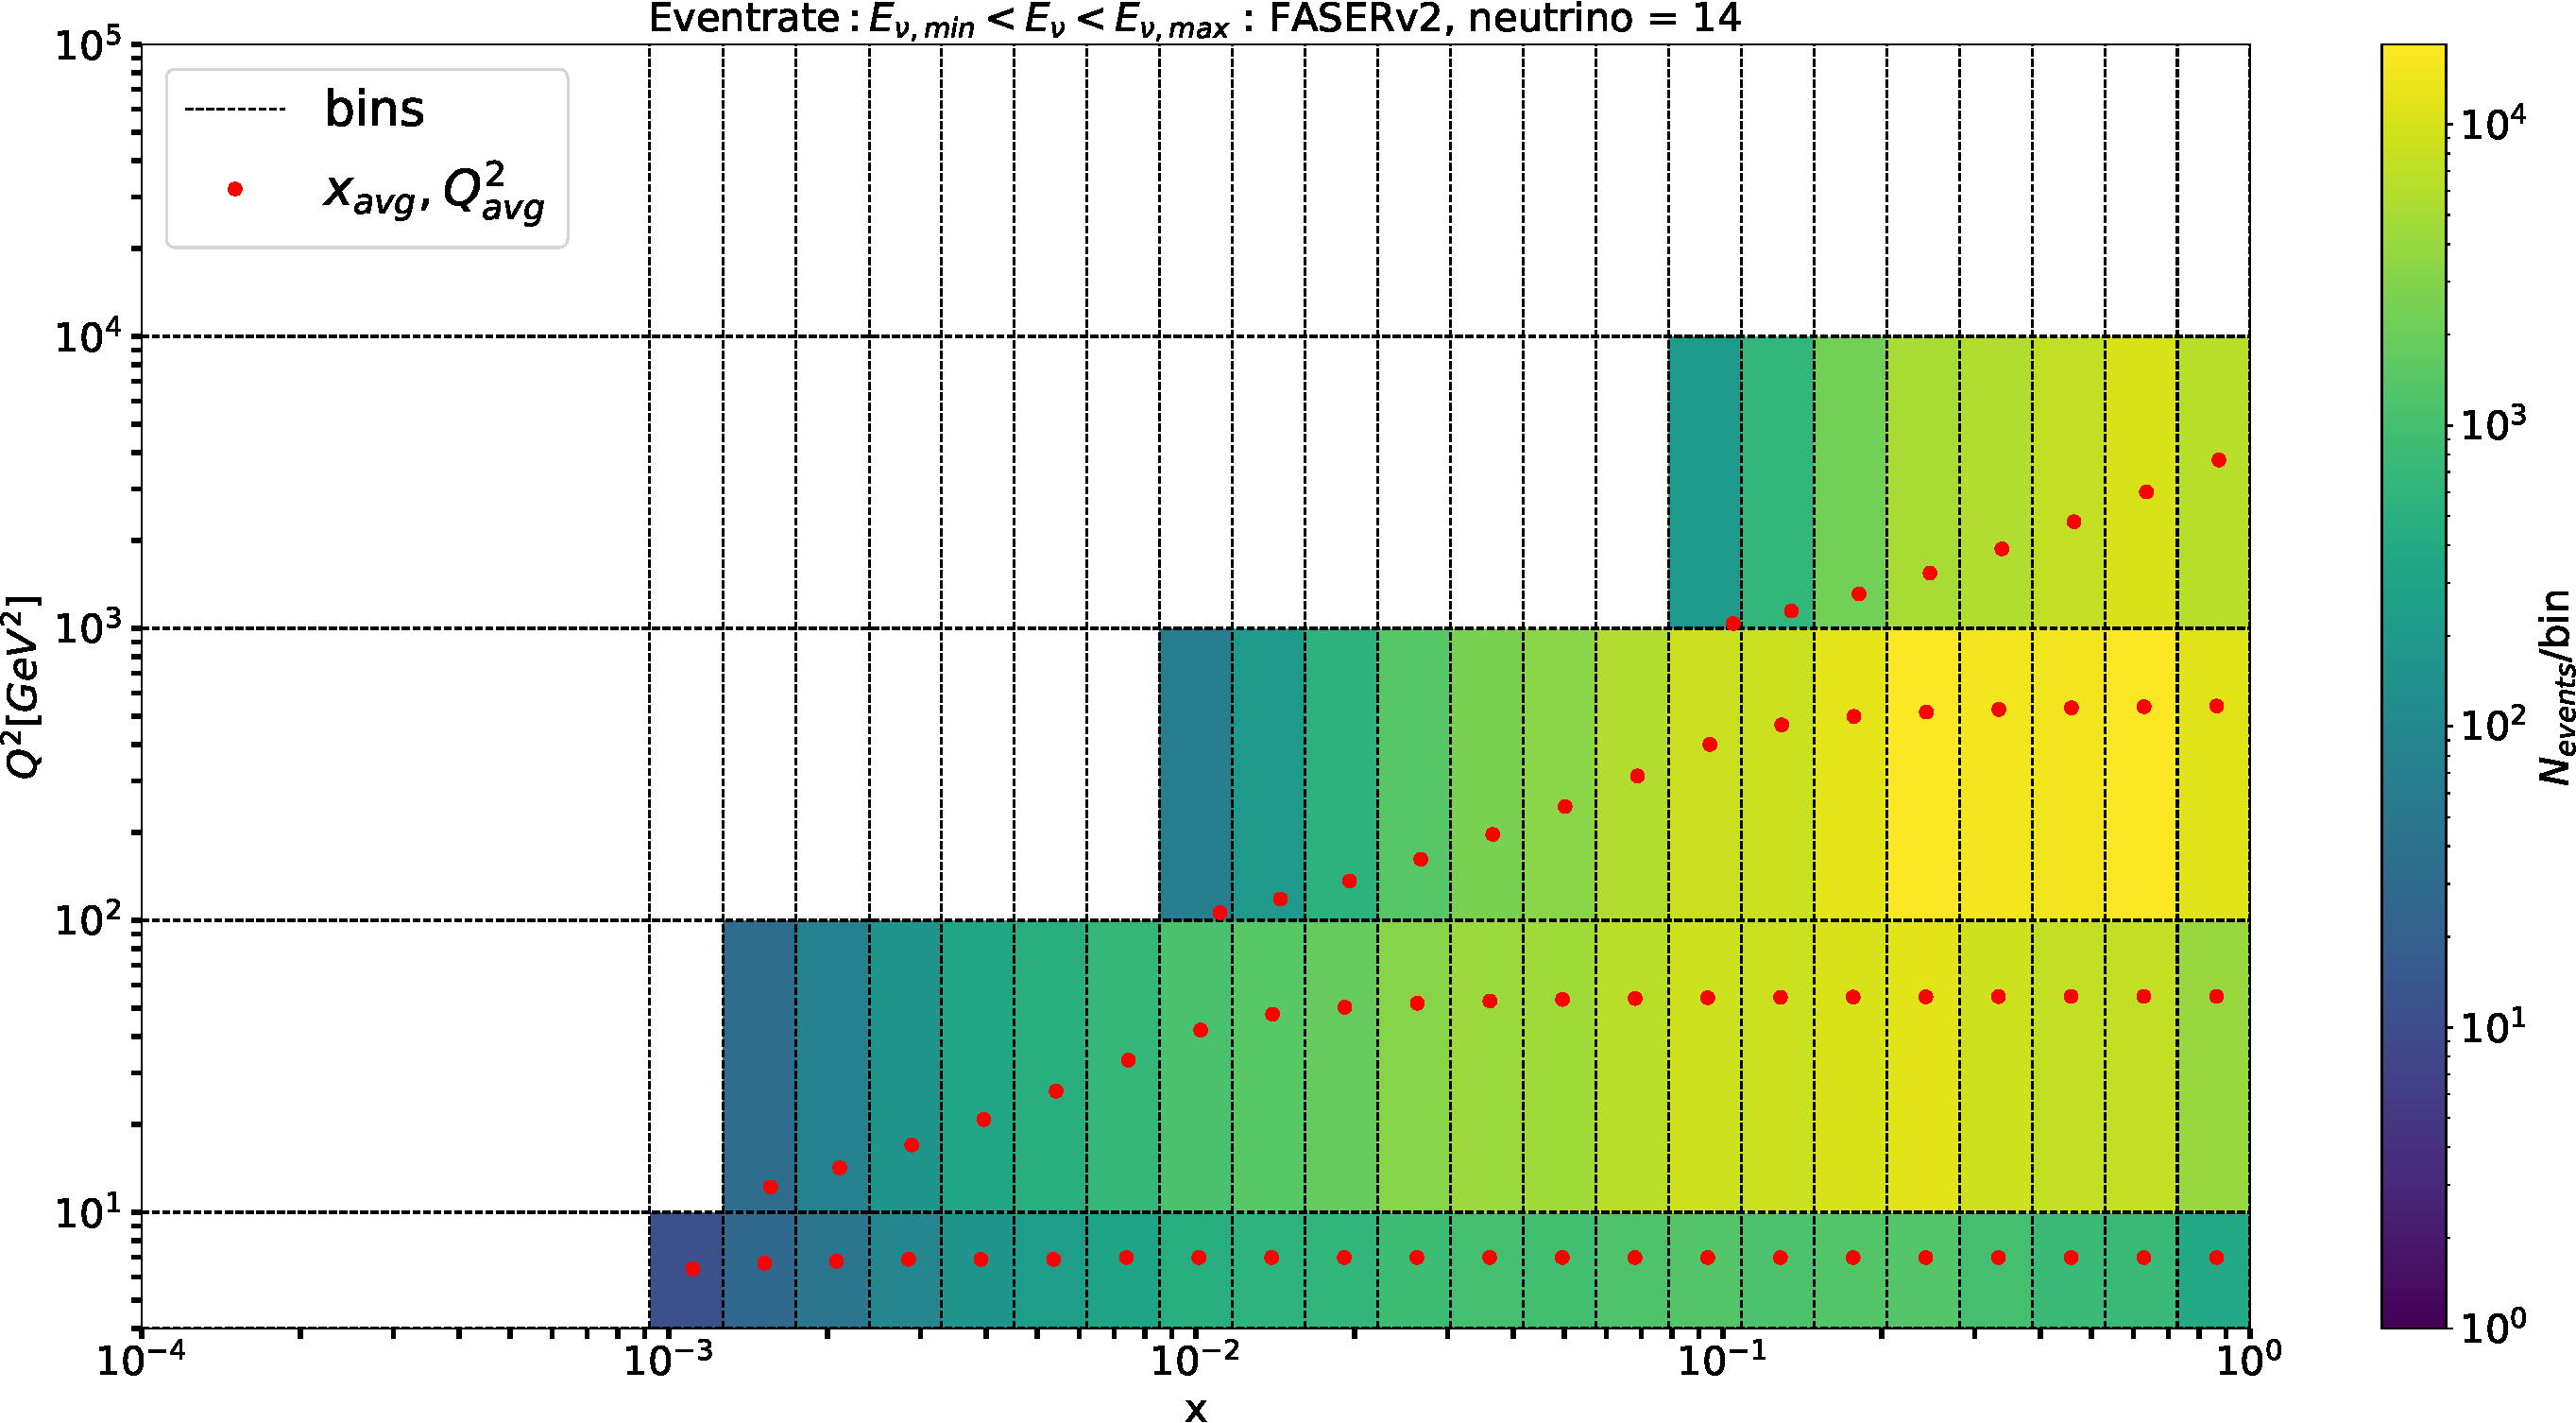
\includegraphics[width=0.9\textwidth]{plots/Nevent_FASERv2_14.pdf}
\caption{\small The event yields per bin $ N_{\rm ev}^{(i)}$,  Eq.~(\ref{eq:event_yields}),
  for muon neutrinos at FASER$\nu$2.
  %
  We present results binned in $x$ and $Q^2$ and integrating over the neutrino energies.
  %
  The red dot indicates the weighted center of each bin.
  %
  Adding up all bin entries results into $N_{\rm ev}(\nu_\mu)\sim 3\times 10^5 $ reconstructed muon
  neutrinos. }
    \label{fig:fasernu2_muon}
\end{figure}
%-----------------------------------------------------------------------

Fig.~\ref{fig:percentage_error_elepton}
displays the estimated systematic uncertainties for the  measurements
of the double-differential
neutrino scattering cross-section at FASER$\nu$2.
%
We consider the leading sources of systematic errors,
associated respectively to the charged lepton energy $E_\ell$ and scattering angle $\theta_\ell$
and to the hadronic energy $E_h$.
%
The size of each source of systematic error is plotted as a function
of the average momentum fraction per bin $\la x\ra$
in three different bins of $Q^2$.
%
We indicate separately the results for neutrino and antineutrino projectiles as well as
those associated to inclusive and to charm production measurements.
%
Systematic uncertainties associated to the hadronic final state energy $E_h$ appear to be the largest.
%
The uncertainties associated to the charged lepton energy $E_\ell$ and scattering angle $\theta_\ell$ range
between a few percent up to 20\% in the nominal baseline scenario,
and in the case of the latter they are the smallest in the large-$x$ region.
%
Similar overview plots have been produced for the other LHC neutrino experiments
considered in this work.

%-----------------------------------------------------------------------
\begin{figure}[!ht]
  \centering
  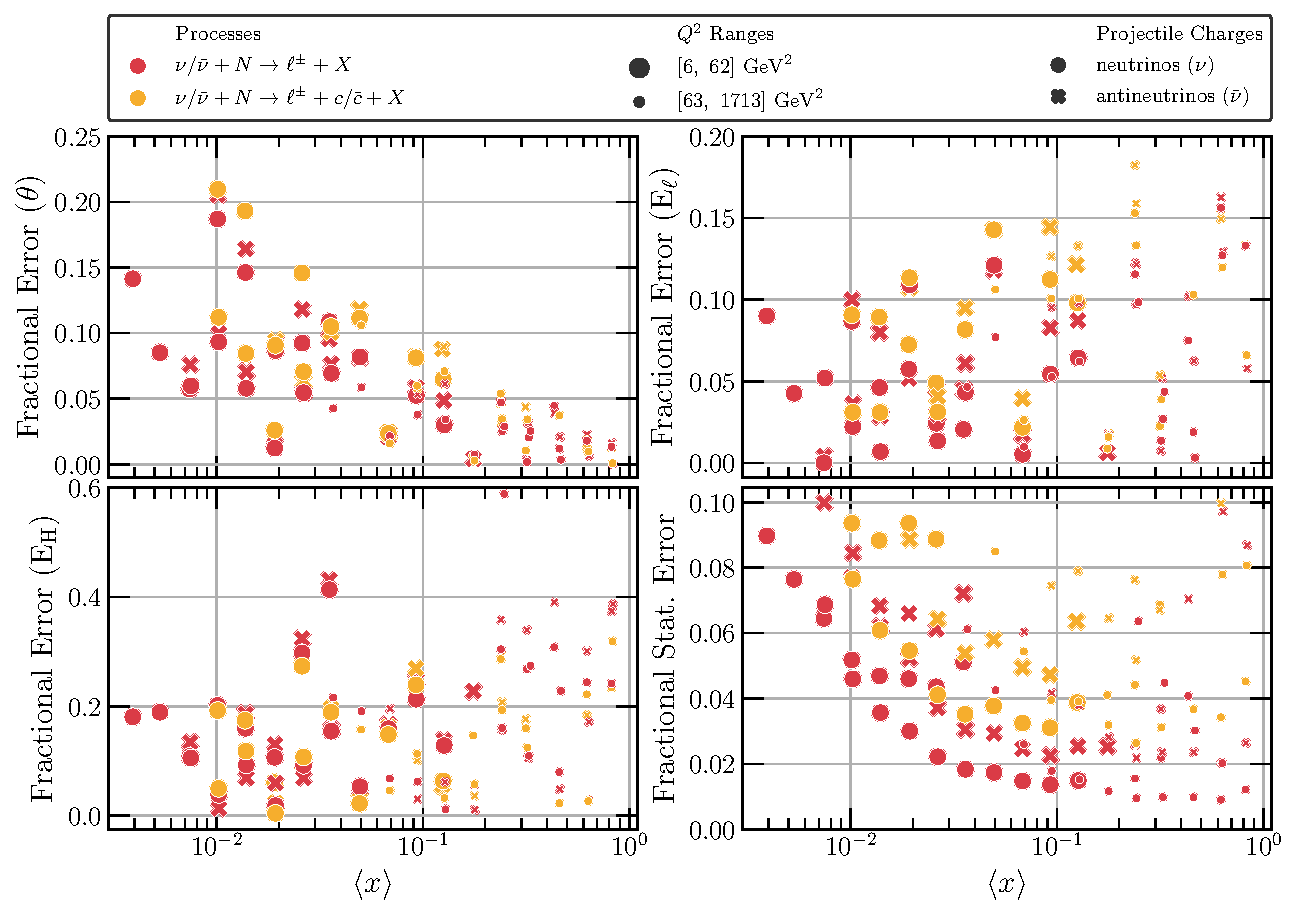
\includegraphics[width=\textwidth]{plots/percentage_errors.pdf}
  \caption{\small Estimated systematic uncertainties for the  measurements
    of the double-differential
    neutrino scattering cross-section at FASER$\nu$2.
    %
    We consider the leading sources of systematic errors,
    associated respectively to the charged lepton energy $E_\ell$ and scattering angle $\theta_\ell$
    and to the hadronic energy $E_h$.
    %
    The size of each source of systematic error is plotted as a function
    of the average momentum fraction per bin $\la x\ra$
    in three different bins of $Q^2$.
    %
    We indicate separately the results for neutrino and antineutrino projectiles as well as
    those associated to inclusive and to charm production measurements.
  }
  \label{fig:percentage_uncertainties_overview}
\end{figure}
%-----------------------------------------------------------------------

The event yields displayed in Fig.~\ref{fig:fasernu2_muon} determine the associated
statistical uncertainty in each bin
\be
\label{eq:statistical_uncertainties}
\delta_{\rm stat}  N_{\rm ev}^{(i)} = \sqrt{N_{\rm ev}^{(i)}} \, ,
\ee
such that the fractional statistical uncertainty per bin is $1/\sqrt{N_{\rm ev}^{(i)}}$.
%
Since here we discard bins with less than 30 events, this statistical uncertainty
ranges between $\sim 1\%$ and $\sim 18\%$ for muon neutrinos in FASER$\nu$2 depending on the values of
$x$ and $Q^2$ associated to this bin.
%
These statistical uncertainties are displayed in the left panel
of Fig.~\ref{fig:error_plot_FASERv2_14}, which corresponds
to the same event yields as in
Fig.~\ref{fig:fasernu2_muon}
now as a function of $x$ after having integrated the event yields in the range $Q^2 \in [10,100]$ GeV$^2$.
%
The error bar in the $y$-direction indicates the statistical uncertainties, while
that in the $x$ direction corresponds to the width of the $x$-bins. {\color{red}[Suggestion (TM): let's refer to horizontal and vertical directions, since $x$ and $y$ are variables as well, not only directions]}

%%%%%%%%%%%%%%%%%%%%%%%%%%%%%%%%%%%%%%%%%%%%%%%%%%%%%
\begin{figure}[h]
    \centering
    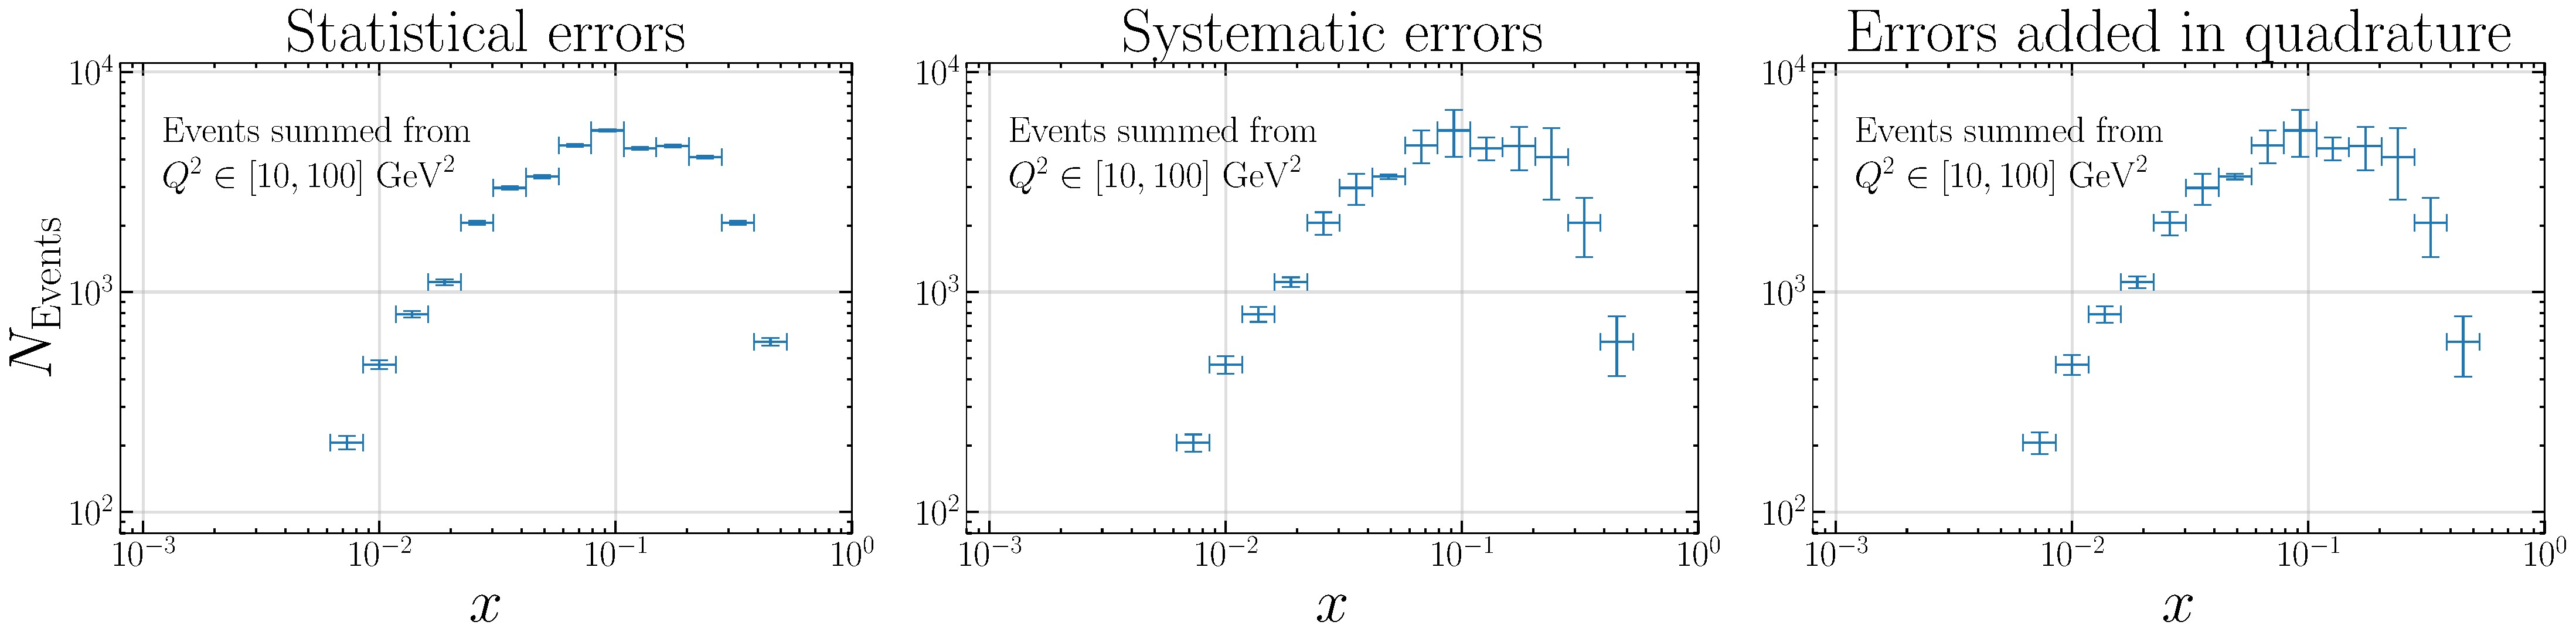
\includegraphics[width = 0.95\textwidth]{plots/error_plot_FASERv2_14.pdf}
    \caption{Same as Fig.~\ref{fig:fasernu2_muon}
      now as a function of $x$ after having integrated the event yields in the range $Q^2 \in [10,100]$ GeV$^2$.
      %
      In addition to the event yields we show the error bars corresponding to
      statistical errors only (left), systematic errors only (middle), and the
      sum in quadrature of the two (right panel).
      %
      The error bars in the $x$ direction indicate the width of the adopted $x$-bins.
      }
    \label{fig:error_plot_FASERv2_14}
\end{figure}
%%%%%%%%%%%%%%%%%%%%%%%%%%%%%%%%%%%%%%%%%%%%%%%%%%%%%%%%%%%%%

Finally, we would like to compare the kinematic reach
of the LHC neutrino measurements with respect to that of other experiments.
%
Fig.~\ref{fig:Kin_nNNPDF30_EIC_FPF} displays
the kinematic coverage of the FASER$\nu$2 experiment in the $(x,Q^2)$ plane,
same as  Fig.~\ref{fig:error_plot_FASERv2_14} now removing bins
containing less than 30 reconstructed events.
%
It is compared to that of electron-ion collisions
at the EIC for the highest center-of-mass energies $\sqrt{s}$ planned,
as well as to the kinematic coverage of other available hard-scattering datasets involving
nuclear targets or projectiles.
%
Specifically, we display the coverage of fixed-target neutral- and charged-current nuclear DIS,
fixed-target Drell-Yan production, and $W$, $Z$, $D$-meson, photon, and dijet
production in proton-lead collisions at the LHC.

%%%%%%%%%%%%%%%%%%%%%%%%%%%%%%%%%%%%%%%%%%%%%%%%%%%%%
\begin{figure}[h]
    \centering
    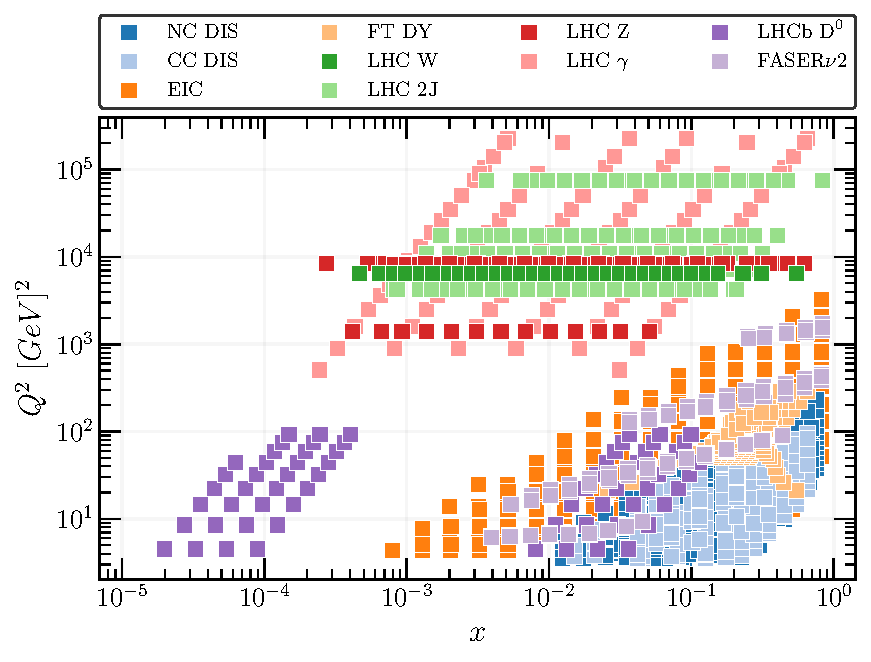
\includegraphics[width = 0.8\textwidth]{plots/Kin_nNNPDF30_EIC_FPF.pdf}
    \caption{The kinematic coverage of the FASER$\nu$2 experiment in the $(x,Q^2)$ plane,
      same as  Fig.~\ref{fig:error_plot_FASERv2_14} now removing bins
      containing less than 30 reconstructed events.
      %
      It is compared to that of electron-ion collisions
      at the EIC for the highest center-of-mass energies $\sqrt{s}$ planned,
      as well as to the kinematic coverage of other available hard-scattering datasets involving
      nuclear targets or projectiles.
      %
      Specifically, we display the coverage of fixed-target neutral- and charged-current nuclear DIS,
      fixed-target Drell-Yan production, and $W$, $Z$, $D$-meson, photon, and dijet
      production in proton-lead collisions at the LHC.
      }
    \label{fig:Kin_nNNPDF30_EIC_FPF}
\end{figure}
%%%%%%%%%%%%%%%%%%%%%%%%%%%%%%%%%%%%%%%%%%%%%%%%%%%%%%%%%%%%%


\subsection{Systematic uncertainties}
\label{sec:systematic_uncertainties}

In addition to the statistical uncertainties given by Eq.~(\ref{eq:statistical_uncertainties}),
one needs to estimate the systematic uncertainties associated to the reconstruction
of the final state leptonic and hadronic variables as listed in Table~\ref{tab:FPF_experiments}.
%
For instance, an event which would be classified in a given bin in the case
of a perfect detector may end up in a different bin in the presence of systematic
shifts associated to the lepton energy $E_\ell$, lepton scattering angle $\theta_\ell$, and
hadronic energy $E_h$.
%
Hence, for each source of experimental systematic uncertainty we would like to estimate
its impact at the level of event yields and eventually stablish also the associated
correlation matrix.

By means of tree-level DIS kinematics, one can relate the variables describing the neutrino-nucleon
hard-scattering, $(x,Q^2,E_{\nu})$,
with those describing the leptonic and hadronic final state, namely $\lp E_{\ell},\theta_\ell, E_{h} \rp$,
and that correspond to experimentally measured quantities.
%
The mapping between the two sets of variables is 
\bea
E_{\nu} &=& E_\ell + E_h \, ,\nonumber \\
Q^2 &=& 4E_\ell E_{\nu}\sin^2\lp {\theta_\ell/2}\rp  =  4E_\ell \lp E_\ell + E_h  \rp\sin^2\lp {\theta_\ell/2}\rp \, , \\
x &=& \frac{Q^2}{2m_N(E_{\nu} - E_\ell)} = \frac{4E_\ell \lp E_\ell + E_h  \rp\sin^2\lp {\theta_\ell/2}\rp}{2m_NE_{h}} \, , \nonumber
\eea
highlighting how the measurement of $E_{\ell}$, $\theta_\ell$, and $E_{h}$ uniquely specify the hard-scattering
kinematics $(x,Q^2,E_{\nu})$ of the event.
%
Therefore, systematic shifts in the measurement of these final-state variables will modify
the assignment of each event to a given bin of $x$, $Q^2$, and $E_\mu$, introducing a systematic
error in the event yields and hence in the measurement of the double-differential
neutrino scattering cross-section.

In order to determine these bin-by-bin systematic uncertainties,
we extend the calculation delineated in Eq.~(\ref{sec:pseudo-data_generation}) as follows.
%
Let us consider for illustrative purposes the FASER${\nu}$2 case.
%
From Table~\ref{tab:FPF_experiments}, one reads that the corresponding acceptances
and performance parameters for $E_{\ell}$, $\theta_\ell$, and $E_{h}$   are given by
\bea
E_\ell \ge 100~{\rm GeV} \, , \quad \delta E_\ell \sim 30\% \, ,\nonumber \\
E_h \ge 100~{\rm GeV} \, , \quad \delta E_h \sim 30\% \, ,\\
 \theta_\ell \le \tan^{-1}(0.5) \, , \quad \delta\theta_\ell \sim 1~{\rm mrad} \, . \nonumber 
\label{fasernu2systematic_errors}
\eea
In order to translate the systematic uncertainties $\delta E_\ell$, $\delta E_h $,
and $\delta\theta_\ell$ into systematic errors associated to the binned event yields, 
\be
\label{eq:event_yields_systematic_error}
\delta_{\rm sys}^{(E_\ell)} N_{\rm ev}^{(i)} \, ,\quad
\delta_{\rm sys}^{(E_h)} N_{\rm ev}^{(i)}
\, ,\quad
\delta_{\rm sys}^{(\theta_\ell)} N_{\rm ev}^{(i)} \, ,\qquad i=1,\ldots,N_{\rm bin} \, ,
\ee
we generate first a Monte Carlo set of events, denoted by $\mathcal{D}_0$,
composed by $N_{\rm mc} = 10^7$ samples and determine the assignment of each event
to a point in the $\lp x,Q^2,E_{\nu}\rp$ space.
%
By integrating over this sample by means of Eq.~(\ref{MCintegration}) we determine
the binned event yields for this reference $\mathcal{D}_0$ sample.

We then produce a second Monte Carlo sample $\mathcal{D}_1$ starting from the events
of $\mathcal{D}_0$ which are then smeared with Gaussian distributions whose variances
are given by Eq.~(\ref{fasernu2systematic_errors}).
%
The bin assignment of the events in the smeared sample $\mathcal{D}_1$ will
in general be different from those of the baseline sample.
%
The procedure is repeated $M$ times, leading to
$\mathcal{D}_k$ (with $k=1,\ldots,M$) smeared
samples each one leading to a different binned event yields
$ N_{\rm ev}^{(i)(k)}$.
%
Provided the number of samples $M$ is large enough, the standard deviation over samples in this $ N_{\rm ev}^{(i)(k)}$
distribution provides the sought-for estimate of the systematic uncertainties.
%
Furthermore, 
since the systematic errors are treated as uncorrelated among them,
by producing samples where only one source of error is varied at a time
we can determine the values of Eq.~(\ref{eq:event_yields_systematic_error}) in each bin.

The end result of the procedure is the estimate of statistical and systematic uncertainties
for each bin of the measurement, from which a experimental covariance matrix can be constructed as
\be
   {\rm cov}_{ij} = \delta_{ij} \lp \delta_{\rm stat}  N_{\rm ev}^{(i)}\rp^2
   + \lp \delta_{\rm sys}^{(E_\ell)} N_{\rm ev}^{(i)} \rp \lp \delta_{\rm sys}^{(E_\ell)} N_{\rm ev}^{(j)} \rp 
   + \lp \delta_{\rm sys}^{(E_h)} N_{\rm ev}^{(i)} \rp \lp\delta_{\rm sys}^{(E_h)} N_{\rm ev}^{(j)}\rp 
   + \lp \delta_{\rm sys}^{(\theta_\ell)} N_{\rm ev}^{(i)} \rp
   \lp \delta_{\rm sys}^{(\theta_\ell)} N_{\rm ev}^{(j)} \rp
   \, ,\qquad
 \nonumber
 \ee
 for $i,j=1,\ldots,N_{\rm bin}$, and the same for the associated correlation
 matrix of the measurement
 \be
 \rho_{ij} =  \frac{{\rm cov}_{ij}}{\sqrt{ {\rm cov}_{ii} }\sqrt{ {\rm cov}_{jj} } } \, . 
 \ee
 The relative covariance matrix, $ {\rm cov}_{ij}/( N_{\rm ev}^{(i)}N_{\rm ev}^{(j)})$, is
 independent of the considered observable and would also apply
 for the double-differential cross-sections Eqns.~(\ref{eq:neutrino_DIS_xsec_FL}) and~(\ref{eq:antineutrino_DIS_xsec_FL}) which are related to the event yields by a constant factor.
 
 One should emphasize that in a real experiment the actual covariance matrix will be
 composed by a much larger number of uncertainty sources, with typical
  HERA and LHC precision measurements characterised by up to hundreds
 of different sources of systematic error.
 %
 In particular, the assumption that a single source of systematic error, say $\delta E_\ell$,
 is fully correlated among all the bins in $(x,Q^2)$ is likely not to be realistic.
 %
 For this reason, here we present impact results both for the nominal correlation model,
 for the case where systematic and statistical uncertainties are added in quadrature,
 and intermediate scenarios.
  
 Fig.~\ref{fig:error_plot_FASERv2_14} (central and right panels) display
 the integrated event yields for FASER$\nu$2 as a function of $x$ for only
 systematic errors and for the sum in quadrature of statistical and systematic errors.
 %
 For most of the bins, for the baseline performance assumptions the total systematic
 uncertainty is at the $10\%$ and dominates over the statistical uncertainties.
 
 \subsection{Pseudo-data generation}

 In order to generate pseudo-data for double-differential
 neutrino scattering cross-sections at the LHC, we follow the procedure
 used for the HL-LHC PDF projections of~\cite{AbdulKhalek:2018rok} which was
 also adopted in~\cite{Ethier:2021ydt} and~\cite{Greljo:2021kvv} for SMEFT impact projections
 of vector-boson scattering and high-mass Drell-Yan data at the HL-LHC, respectively.
 %
 The starting point are the predictions for the differential neutrino scattering
 cross-section
 \be
 \label{eq:theory_dis_projections}
 \mathcal{O}_i^{{\rm (th)}} \equiv \frac{d^2\sigma^{\nu N}(x_i,Q^2_i,y_i)}{dxdy} \, ,\quad
 i=1,\ldots,N_{\rm bin} \, ,
 \ee
 with $(x_i,Q^2_i,y_i)$ being the corresponding bin centers.
 %
 The observables $\mathcal{O}_i $ are evaluated using {\sc\small YADISM} and {\sc\small PineAPPL}
 as described in Sect.~\ref{sec:settings}.
 %
 An important point here is the choice of PDF set entering the evaluation of
 the observable in Eq.~(\ref{eq:theory_dis_projections}): it should be consistent
 with that of the fitting framework used to assess their impact on the (n)PDFs.
 %
 For instance, when using the {\sc\small xFitter} profiling of PDF4LHC21, one needs
 to generate LHC neutrino pseudo-data also using PDF4LHC21 as input.
 %
 In order words, the generated pseudo-data should be fully consistent with the prior PDF
 set used as baseline, else one is introducing artificially inconsistencies which
 compromise the validity of the projection studies.
 
 The central values for the LHC neutrino scattering pseudo-data, denoted
 by $\mathcal{O}_i^{{\rm (exp)}} $, are obtained
 by fluctuating this reference theory prediction by the statistical and systematic
 uncertainties, that is
 \begin{equation}
  \label{eq:pseudo_data}
  \mathcal{O}_i^{{\rm (exp)}}
  =   \mathcal{O}_i^{{\rm (th)}}\left( 1+ r_{i} \delta_{i}^{\rm stat}
  + \sum_{k=E_\ell, E_h,\theta_\ell}
    r'_{k} \,\delta_{i,k}^{{\rm sys}}\right) \, , \qquad i=1,\ldots,N_{\rm bin} \, ,
 \end{equation}
 with $r_{i}$ and $r'_{k}$ being univariate Gaussian random numbers,
 and $\delta_i^{\rm stat}$ ($\delta_{i,k}^{\rm sys}$) indicate the relative statistical (systematic)
 uncertainties associated to the $i$-th bin (and $k$-th source of systematic uncertainty).
 %
 Note that a given systematic variation is assumed to be fully correlated among all the bins
 in the measurement.

 Alternatively, we can add all uncertainties in quadrature and account for a possible
 improvement in the systematic errors with respect to the current estimates,
 \be
 \delta_{i}^{\rm tot}
 = \left( \left( \delta_i^{\rm stat}\right)^2 + \sum_{k=1}^{n_{\rm sys}}
\left( \delta_{i,k}^{\rm sys} \right)^2\right)^{1/2} \, ,
 \ee
 and the pseudo-data is evaluated by means of
 \begin{equation}
  \label{eq:pseudo_data_v2}
  \mathcal{O}_i^{{\rm (exp)}}
  = \mathcal{O}_i^{{\rm (th)}}
    \left( 1+ r_i \delta_i^{\rm tot}
    \right) \,
    , \qquad i=1,\ldots,N_{\rm bin} \, .
 \end{equation}
 While the actual correlation model will lie somewhere between no correlation and full correlation,
 these two approaches to generate the pseudo-data bracket the projected impact
 on the PDFs and its dependence on the experimental correlation model.
 
